\documentclass[12pt, titlepage]{article}

\usepackage{booktabs}
\usepackage{tabularx}
\usepackage{hyperref}

\usepackage{fullpage}
\usepackage[round]{natbib}
\usepackage{multirow}
\usepackage{booktabs}
\usepackage{tabularx}
\usepackage{graphicx}
\usepackage{float}
\usepackage{hyperref}
\usepackage{colortbl}
\usepackage[table]{xcolor} 
\hypersetup{
    colorlinks,
    citecolor=black,
    filecolor=black,
    linkcolor=red,
    urlcolor=blue
}
\usepackage[round]{natbib}

%% Comments

\usepackage{color}

%\newif\ifcomments\commentstrue %displays comments
\newif\ifcomments\commentsfalse %so that comments do not display

\ifcomments
\newcommand{\authornote}[3]{\textcolor{#1}{[#3 ---#2]}}
\newcommand{\todo}[1]{\textcolor{red}{[TODO: #1]}}
\else
\newcommand{\authornote}[3]{}
\newcommand{\todo}[1]{}
\fi

\newcommand{\wss}[1]{\authornote{blue}{SS}{#1}} 
\newcommand{\plt}[1]{\authornote{magenta}{TPLT}{#1}} %For explanation of the template
\newcommand{\an}[1]{\authornote{cyan}{Author}{#1}}

%% Common Parts

\newcommand{\progname}{Mechatronics Engineering} % PUT YOUR PROGRAM NAME HERE
\newcommand{\authname}{Team 25, Preliminary
\\ Ahmed Nazir, nazira1
\\ Stephen Oh, ohs9
\\ Muhanad Sada, sadam
\\ Tioluwalayomi Babayeju, babayejt} % AUTHOR NAMES                  

\usepackage{hyperref}
    \hypersetup{colorlinks=true, linkcolor=blue, citecolor=blue, filecolor=blue,
                urlcolor=blue, unicode=false}
    \urlstyle{same}
                                


\begin{document}

\title{Verification and Validation Report: \progname} 
\author{\authname}
\date{\today}
	
\maketitle

\pagenumbering{roman}

\section{Revision History}

\begin{tabularx}{\textwidth}{p{3cm}p{2cm}X}
\toprule {\bf Date} & {\bf Version} & {\bf Notes}\\
\midrule
Date 1 & 1.0 & Notes\\
Date 2 & 1.1 & Notes\\
\bottomrule
\end{tabularx}

~\newpage

\section{Symbols, Abbreviations and Acronyms}

\renewcommand{\arraystretch}{1.2}
\begin{tabular}{l l} 
  \toprule		
  \textbf{symbol} & \textbf{description}\\
  \midrule 
  T & Test\\
  \bottomrule
\end{tabular}\\

\wss{symbols, abbreviations or acronyms -- you can reference the SRS tables if needed}

\newpage

\tableofcontents

\listoftables %if appropriate

\listoffigures %if appropriate

\newpage

\pagenumbering{arabic}

This document ...

\section{Functional Requirements Evaluation}
%sensor validation: Stephen
\begin{table}[!htbp]
  \begin{tabular}{| p{0.13\textwidth} | p{0.10\textwidth}| p{0.28\textwidth}| p{0.28\textwidth}| p{0.10\textwidth}|}
    \hline
    \rowcolor[gray]{0.9}
    Test Number & Type & Input & Output & Result\\
    \hline
    ST-SV 1 & Manual & Room at a constant 25 $^{\circ}$C ambient & Constant 25.4 $^{\circ}$C reading from temperature sensor & Pass \\
    \hline
    ST-SV 2 & Manual & Room at constant 40\% humidity $^{\circ}$C & Constant 43\% reading from humidity sensor & Pass \\
    \hline
    ST-SV 3 & Manual & 4 seperate phonecalls with accelerometer measuring haptic feedback & Maximum error between acceleration profiles of phone calls within 0.2 meters per second squared & Pass  \\
    \hline
  \end{tabular}
  \caption{Sensor Validation}
  \end{table}

%device telemetry: Ahmed
%device hardware: Stephen
\begin{table}[!htbp]
  \begin{tabular}{| p{0.13\textwidth} | p{0.10\textwidth}| p{0.28\textwidth}| p{0.28\textwidth}| p{0.10\textwidth}|}
    \hline
    \rowcolor[gray]{0.9}
    Test Number & Type & Input & Output & Result\\
    \hline
    ST-DH 1 & Manual & Temperature sensor male end JST connector unconnected to the device's female JST connector & Device measured the room's ambient temperature at 23.4 $^{\circ}$C & Pass \\
    \hline
    ST-DH 2 & Manual & Device collecting sensor data at low battery charge & Device unoperational upon battery depletion and halted sensor data collection & Fail \\
    \hline
    ST-DH 3 & Manual & 5 kg dumbbell placed on each corner of the device chassis & No plastic failure in device chassis & Pass  \\
    \hline
    ST-DH 4 & Manual & A member on the formula electric team was given a cross screwdriver, M4 screw, the device, and DIN rail & The formula electric team member mounted the device in 40 seconds & Pass  \\
    \hline
%REMEMBER TO DELETE ST-DH5 FROM VNVPLAN, WE DO NOT NEED THIS TEST AS WE DO NOT HAVE A SCREEN OR DEVICE STATUS MEASUREMENTS
  \end{tabular}
  \caption{Device Hardware}
  \end{table} 
  \newpage 

  ST-DH3 failed the functional test case. The team estimated the time required to design and integrate a rechargeable battery subsystem within the project's timeline was 1.5 weeks and decided the effort was not worthwhile relative to other project objectives. As a result, the failure of this test case lead the expected operation at low battery to be adjusted. Users are now expected to replace the battery on a regular schedule to prevent a failure in test integrity due to charge depletion. \\

%desktop app: Mo
%data analytics: Tio
%database: Mo
\section{Nonfunctional Requirements Evaluation}
\subsection{Usability}
%Stephen
%Need a graph (that we generate) that supports data
\newpage
\begin{table}[h!]
  \begin{tabular}{| p{0.13\textwidth} | p{0.10\textwidth}| p{0.28\textwidth}| p{0.28\textwidth}| p{0.10\textwidth}|}
    \hline
    \rowcolor[gray]{0.9}
    Test Number & Type & Input & Output & Result\\
    \hline
    ST-U 1-A & Manual & User connects a thermistor to device, begins collecting sensor test data and gathers data for 1 minute, completes collecting sensor test data, adds remarks to the test, and submits test data to database & User completed the overall process in 3 minutes 43 seconds and rated the sensor mount and measuring procedure a 5. All other categories were given a 4 & Pass \\
    \hline
    ST-U 1-B & Manual & User adjusts Arduino code for a fluid flow rate sensor, connects the sensor to the device, begins collecting sensor test data and gathers data for 1 minute, completes collecting sensor test data, adds remarks to the test, and submits test data to database & User completed the process in 49 minutes 15 seconds and rated the overall experience a 2. The sensor mount and measuring procedure categories were given a 5. All other cattegories were given a 4 & Fail \\
    \hline
    ST-U 2-A & Manual & Device collecting sensor data with wired connection to a laptop running the python application & Python application GUI displayed at minimal latency. Less than 1 second latency for changes in sensor measurements to display on GUI & Pass \\
    \hline
    ST-U 2-B & Manual & Device collecting sensor data with wireless connection to a laptop running the python application & Python application GUI displayed at minimal latency. Less than 1 second latency for changes in sensor measurements to display on GUI & Pass \\
    \hline
    ST-U 3-A & Manual & Device connection to application is broken. User submits previous test data held on the micro-SD module to the database & Test data submits and test contents can be viewed on dashboard & Pass \\
    \hline
    ST-U 3-B & Manual & Application connection to database is broken. User can connect a temperature sensor, start a test, and stop a test & Device recognizes sensor, starts test, and stops test & Pass  \\
    \hline
  \end{tabular}
  \caption{Usability}
  \end{table}

  \begin{figure}[htbp!]
    \begin{center}
    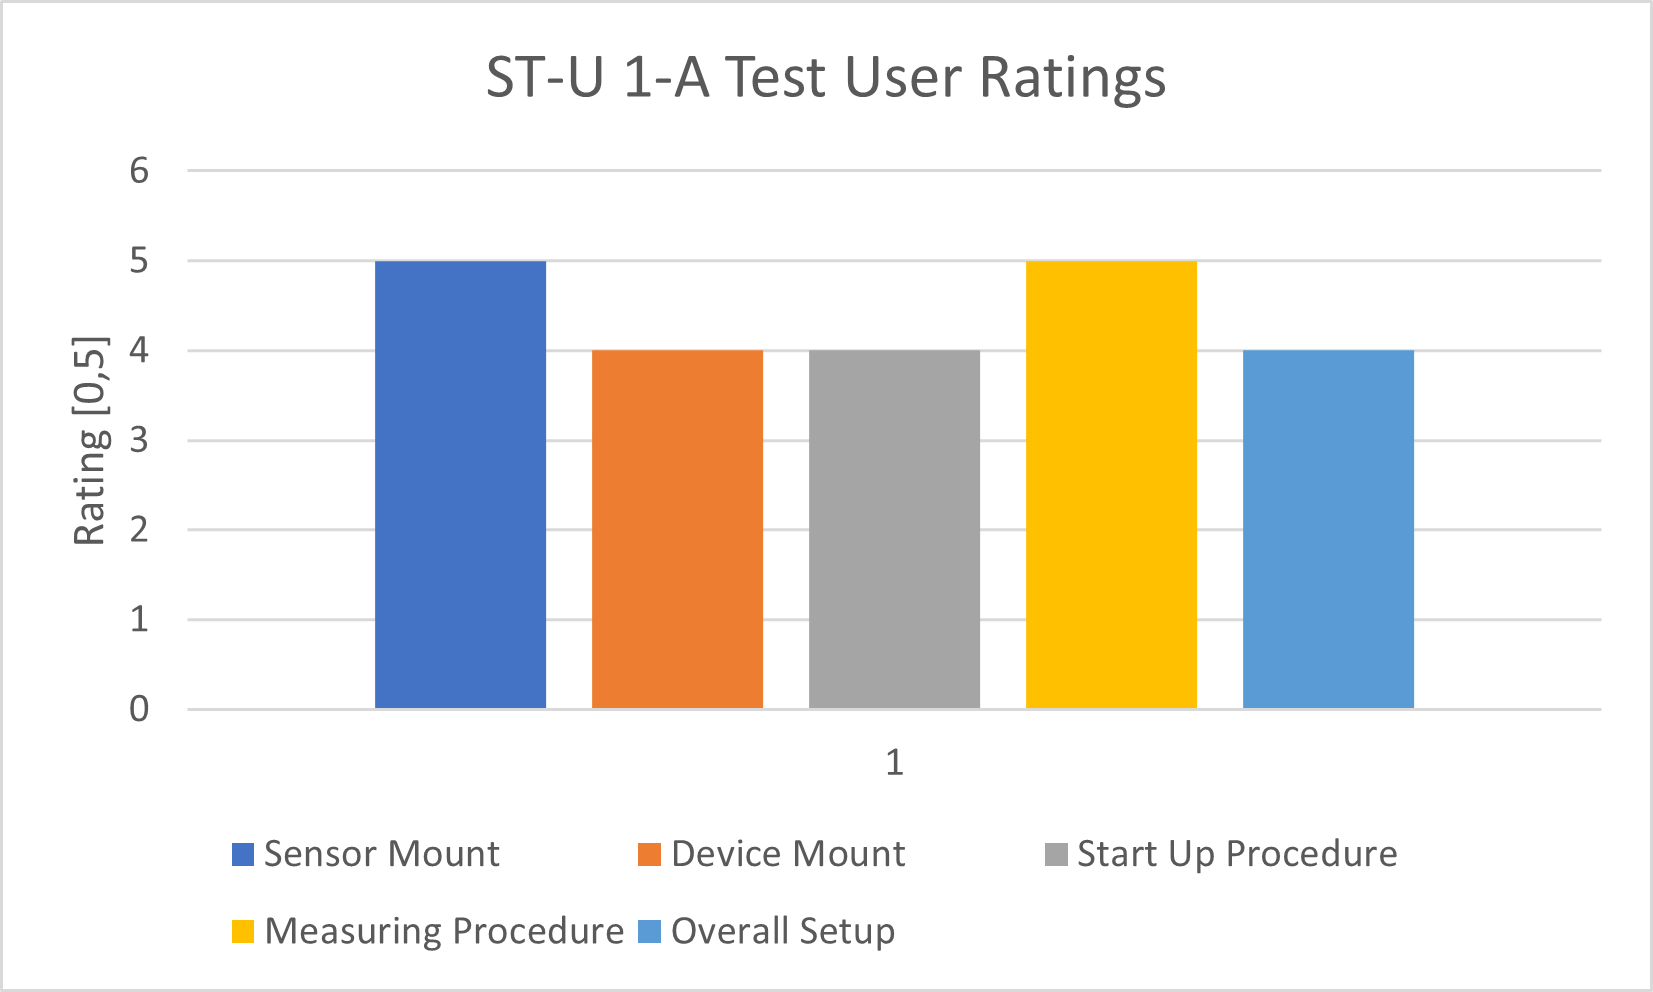
\includegraphics[width=0.8\textwidth]{ST-U_1-A_TestUserRatings}
    \caption{ST-U 1-A Test User Ratings}
    \end{center}
    \end{figure}

  \begin{figure}[htbp!]
    \begin{center}
    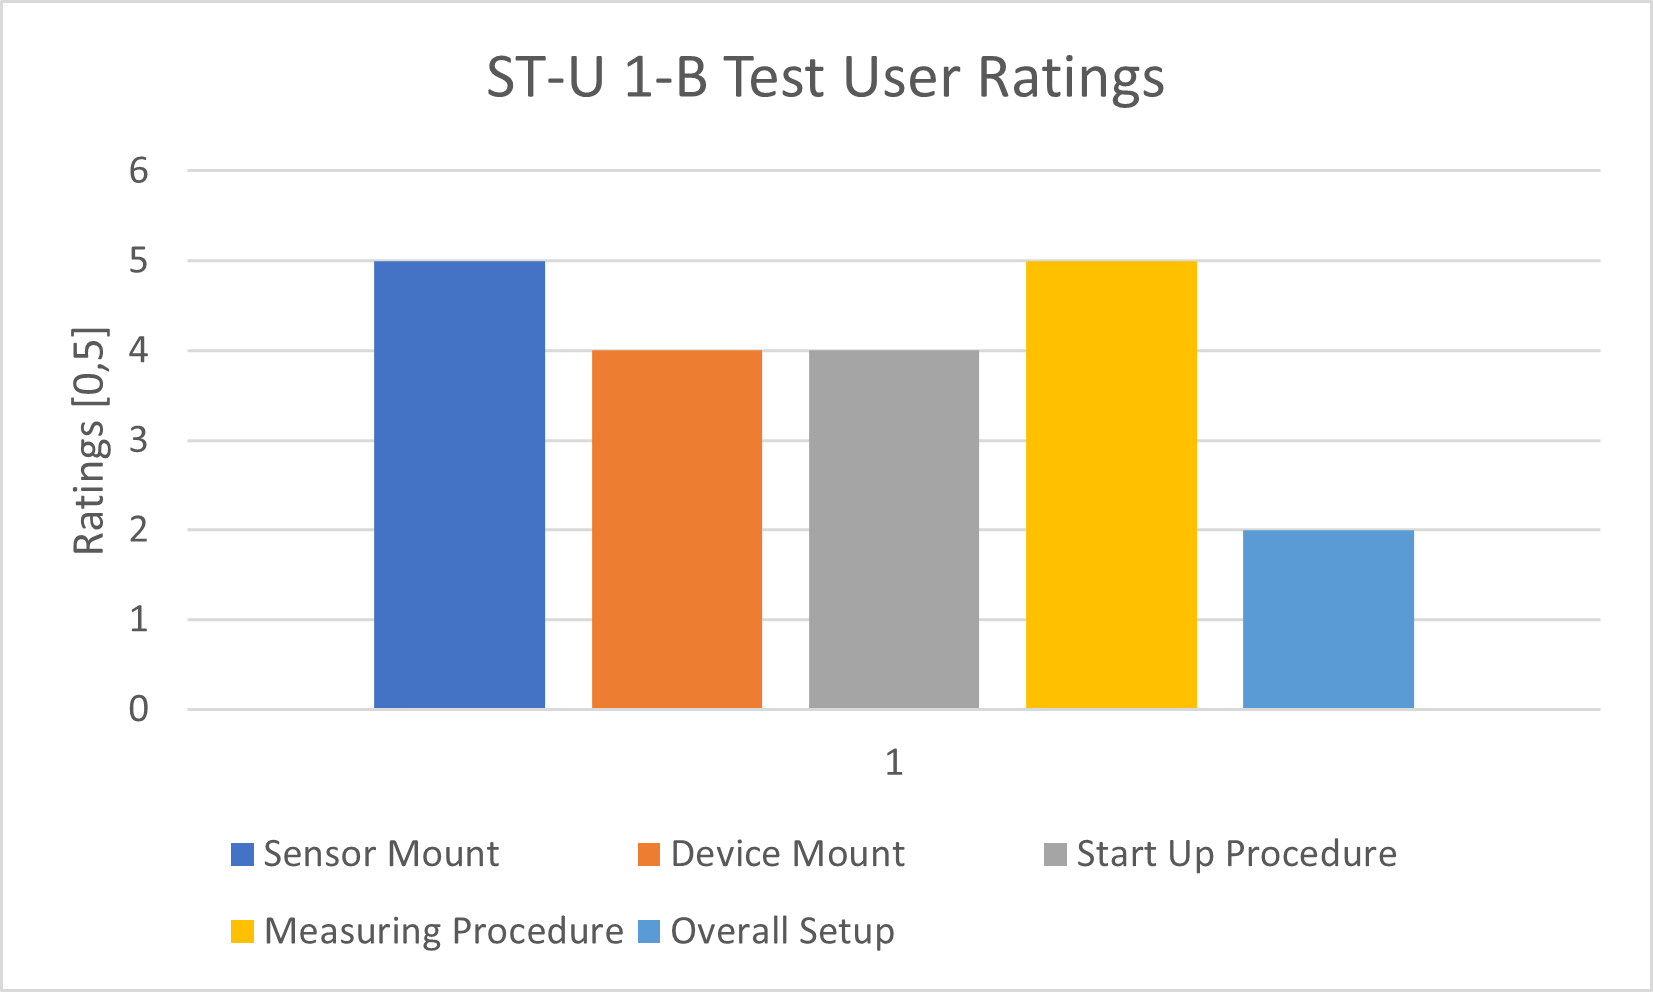
\includegraphics[width=0.8\textwidth]{ST-U_1-B_TestUserRatings}
    \caption{ST-U 1-B Test User Ratings}
    \end{center}
    \end{figure}

  ST-U 1-B failed the usability test case. The difference between ST-U 1-B and ST-U 1-A was the user requirement to adjust and write the Arduino code for a sensor not previously used with the device. Notably, the user experienced difficulty and was intimidated with adjusting existing code to integrate a new sensor. This effect was shown in both the increased time to complete the overall process and the decreased rating in the overall test experience category. As a result, the project will have an approach whereby the user should only interact with the graphical user interface to reduce the user's feelings of complexity and intimidation when integrating a new sensor. The goal is to abstract the adjustments in the backend when implementing a new sensor by having the user interact only with the GUI and following guided steps in plain English to fill in the required information to integrate a new sensor. \\


\subsection{Performance}
%Tio
%Need a graph (that we generate) that supports data 

\subsection{Security}
%Tio

\section{Unit Testing}
%Desktop App Code: Mo
%Arduino Code: Ahmed

\section{Changes Due to Testing}
%Each person will have to write a section here. Each FR and NFR will have a paragraph here, so based on what was assigned earlier, we will need to write a section here.

\subsection{Functional Requirements}
%NOTE: Only keep requirements in here that were changed
%FR 1 :
%Point 1: Changes
%Point 2: Effect the change had on project
FR 11 was changed such that the battery under expected operational use is non-rechargeable. Batteries will continue to be used but will change from rechargeable to non-rechargeable batteries with a scheduled replacement timeline close to charge depletion. This change followed the test ST-DH 2 results. \\

\subsection{Nonfunctional Requirements}

\wss{This section should highlight how feedback from the users and from 
the supervisor (when one exists) shaped the final product.  In particular 
the feedback from the Rev 0 demo to the supervisor (or to potential users) 
should be highlighted.}

Additional considerations to the GUI must be made in response to NFR1,  NFR2, and the test result ST-U 1-B. In particular, the team plans to improve the GUI to improve the user experience by minimizing and ultimately eliminating interaction with Arduino code when integrating new sensors and making the user work with the GUI to integrate new sensors. \\
		
\section{Trace to Requirements}
%VnV Plan has this table
		
\section{Trace to Modules}		
%Mapping unit tests to modules: MG has this table

\bibliographystyle{plainnat}
\bibliography{../../refs/References}

\newpage{}
\section*{Appendix --- Reflection}

The information in this section will be used to evaluate the team members on the
graduate attribute of Reflection.  Please answer the following question:

\begin{enumerate}
  \item In what ways was the Verification and Validation (VnV) Plan different
  from the activities that were actually conducted for VnV?  If there were
  differences, what changes required the modification in the plan?  Why did
  these changes occur?  Would you be able to anticipate these changes in future
  projects?  If there weren't any differences, how was your team able to clearly
  predict a feasible amount of effort and the right tasks needed to build the
  evidence that demonstrates the required quality?  (It is expected that most
  teams will have had to deviate from their original VnV Plan.)

  %Each person has 1 paragraph on stuff they worked that they can comment on. Ideally, 4 paragraphs total

  %Stephen
  The Verification and Validation Plan for usability differed from the actual activities conducted in the VnV. For example, the usability test ST-U 1 did not originally account sensor code integration by the user during the test. But during VnV, the team realized that we needed to know both the total process time taken when the user already had the required code and when the user had to integrate the code to adequately determe the project's ability to meet the FR's and NFR's defined in the SRS. In the future, prototyping earlier in the design process can help identify important test cases when generating the VnV Plan. \\
  %End of paragraph

\end{enumerate}

\end{document}